\Aufgabe[Predicate Abstraction\hfill\textbf{(1.5 Point)}]
Consider the following program:
\begin{verbatim}
void foo(int j, int z) {
  assume(z != 0);
  int i := j;
  while(z != 0) {
      i := i + z;
      if(z > 0)
          z--
      else
          z ++;
  };
  assert(i != j)
}
\end{verbatim}

The {\em assume statement} at the beginning of the function forces the parameter $z$ not to be 0 when the function is called.

\begin{enumerate}

 \item Argue in your own words why the assertion at the end of the program allways holds, i.e., why the error state can never be reached.

 \item Provide a labeled transition system for the given program.

 \item Provide an abstraction for the labeled transition system that uses the predicates $i = j$, $i < j$, $i > j$.

 \item Check whether the error state can be reached in the abstraction, if so state a trace to the error state and refine the abstraction with suitable predicates such that the error state is not reachable anymore.

\end{enumerate}


\textbf{Solution:}\\
\medskip
\begin{enumerate}
\item The call of the method \texttt{\small assume(z != 0)} in the beginning
of the program forces, that the value of the variable $z$ is not $0$. Since
the semantics of \texttt{\small assume(x)}, means that "by assumption \texttt%
{\small x} holds" and by definition an assumption can never being violated.
Thus, the while-loop will be executed at least one time, regardless if the
value of $z$ is positive or negative.

Since the if-condition inside of the loop controls $z$ by decrementing or
incrementing and consequently the variable $i$ will also incremented or
decremented. Thus, the loop will be executed exactly in $|z|$ times. Since  $%
i=j$ is in the precondition of the loop, the loop is guaranteed to terminate
since $z\neq 0$. Hence, after the termination of the while-loop, the case
that $i=j$ will never reached, i.e. it will never hold.

\item
\newpage
\textit{Labeled Transiton System (LTS):}
\begin{figure}[th]
\centering
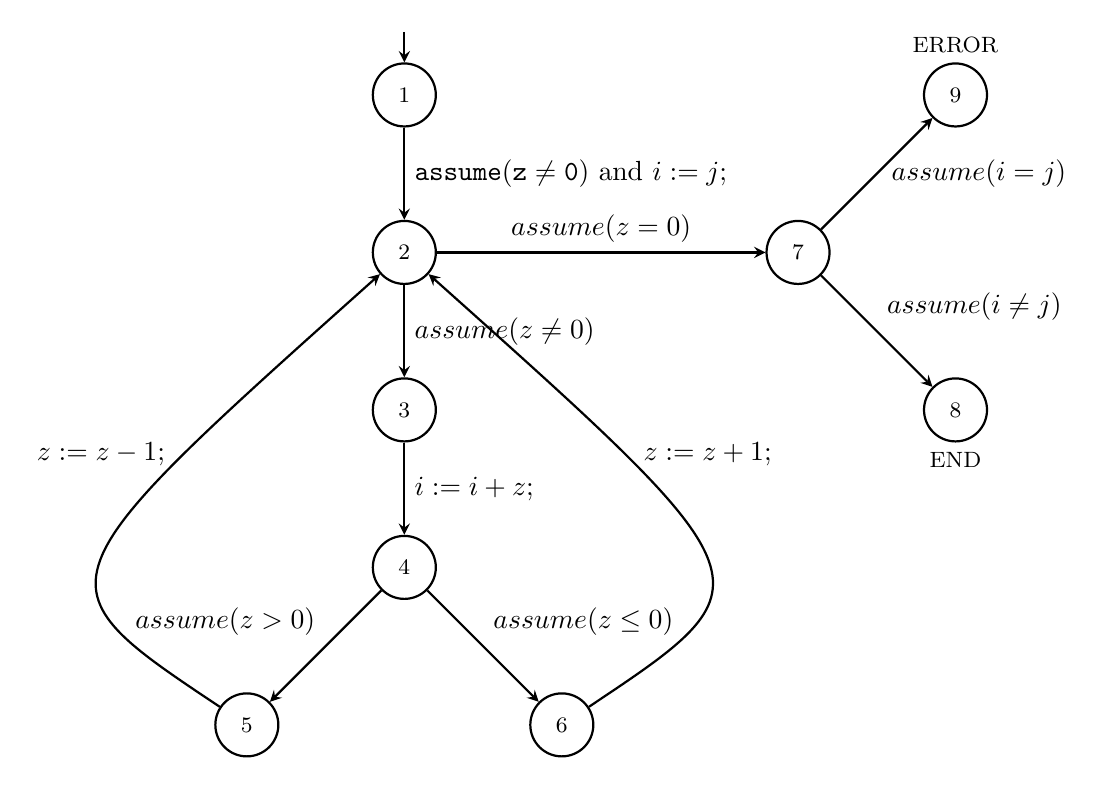
\begin{tikzpicture}[->, >=stealth, line join=bevel]
	\pgfsetlinewidth{1bp}
	\pgfsetcolor{black}

	\tikzstyle{state} = [draw,shape=circle,minimum size=8mm,font=\footnotesize];
	\tikzstyle{accept_state} = [shape=circle, minimum size=8mm, accepting, font=\small, draw];
	\tikzstyle{every path} = [draw, thick];

	\node[state] at (0,10) (1) {$1$};
	\node[state] at (0,8) (2) {$2$}; 
	\node[state] at (0,6) (3) {$3$}; 
	\node[state] at (0,4) (4) {$4$}; 
	\node[state] at (-2,2) (5) {$5$}; 
	\node[state] at (2,2) (6) {$6$}; 
	\node[state] at (5,8) (7) {$7$}; 
	\node[state] at (7,6) (8) [label=below:{\footnotesize END}] {$8$}; 
	\node[state] at (7,10) (9) [label=above:{\footnotesize ERROR}] {$9$}; 

	\draw (0, 10.8) to (1);
	\draw (1) to node[auto] {$\mbox{\fontsize{10}{11}\selectfont $\mathtt{assume(z \neq 0)} \mbox{ and } i := j;$}$} (2);
	\draw (2) to node[auto] {$\mbox{\fontsize{10}{11}\selectfont $assume(z \neq 0)$}$} (3);
	\draw (3) to node[auto] {$\mbox{\fontsize{10}{11}\selectfont $i := i+z;$}$} (4);
	\draw (4) to node[auto, swap] {$\mbox{\fontsize{10}{11}\selectfont $assume(z > 0)$}$} (5);
	\draw (4) to node[auto] {$\mbox{\fontsize{10}{11}\selectfont $assume(z \leq 0)$}$} (6);
	\draw (2) to node[auto] {$\mbox{\fontsize{10}{11}\selectfont $assume(z = 0)$}$} (7);
	\draw (7) to node[auto] {$\mbox{\fontsize{10}{11}\selectfont $assume(i \neq j)$}$} (8);
	\draw (7) to node[right] {$\mbox{\fontsize{10}{11}\selectfont $\,assume(i = j)$}$} (9);
	\draw[->] (5) .. controls (-4.7,3.8) .. (2) node[pos=.75, left] {$z := z-1;\;$};
	\draw[->] (6) .. controls (4.7,3.8) .. (2) node[pos=.75, right] {$\;z := z+1;$};
\end{tikzpicture}
\caption{{\protect\small LTS of the given program.}}
\label{lts_program}
\end{figure}

\item

Notation + Graph folgen noch

\item
There is no reachable error trace in the abstraction.
\end{enumerate}